\documentclass[11pt,a4paper]{article}
\usepackage{float}
\usepackage[utf8]{inputenc}
\usepackage[left=2cm,right=2cm,text={18cm,24cm},top=2cm]{geometry}
\usepackage[czech]{babel}
\usepackage{graphicx}
\usepackage{verbatim}
\usepackage{fancyvrb}
\usepackage{svg}
\usepackage{biblatex}
\usepackage{hyperref}
\usepackage{tabto}
\usepackage{rotating}


\renewcommand{\familydefault}{\sfdefault}

\begin{document}
\begin{titlepage}
	\begin{center}
		% FIT logo
		\includegraphics[scale=0.65]{include/fit.pdf} \\
		
		\vspace{2cm}
		
		\huge{
			\textbf{
				Projektová dokumentace} \\
			Překladač jazyka IFJ22} \\
				                
		\vspace{2cm}
				            
		\Large{
			Tým xstrel03 \\
			Varianta TRP \\
		}
				                
		\vspace{2cm}
				            
		\normalsize{}
		\today{}
				
		\vspace{2cm}
		\begin{tabular}{l l l}
			\textbf{Matyáš Strelec} & \texttt{xstrel03} & \quad 25\% \\
			Ondřej Seidl             & \texttt{xseidl06} & \quad 25\% \\
			Maxmilián Nový          & \texttt{xnovym00} & \quad 25\% \\
			Dominik Klon              & \texttt{xklond00} & \quad 25\% \\
		\end{tabular}
	\end{center}
\end{titlepage}

\pagebreak{}

\tableofcontents

\pagebreak{}

\section{Práce v týmu}
Společně jsme vytvořili návrh modulů a rozhraní pro komunikaci a předávání dat mezi nimi. Každý pracoval na své části,
vzájemně jsme komunikovali postup ostatním, pokud nastaly chyby, byly zaznamenány a později vyřešeny. Pro sdílení kódu a zaznamenávání
chyb byl využit \verb|GitHub|, pro moduly byly vytvořeny samostatné větve, které se slučovaly do hlavní větve, pokud byla funkcionalita vylepšena.
Pravidelně jsme se scházeli prezenčně nebo on-line, abychom ostatní informovali o stavu kódu a domluvili se
na dalším postupu řešení. V poslední fázi jsme náš program testovali vlastními programy v \verb|IFJ22| a pokud jsme narazili na chybu, společně jsme
ji opravili.
\\\\
Jednotlivé části projektu byly rozděleny mezi členy týmu následovně.

\subsection{Rozdělení práce}

\subsubsection*{Matyáš Strelec \texttt}
\begin{itemize}
	\item Lexikální analýza
	\item Syntaktická analýza
\end{itemize}

\subsubsection*{Ondřej Seidl}
\begin{itemize}
	\item Implementace tabulky symbolů
	\item Zpracování výrazů
	\item Precedenční analýza
\end{itemize}

\subsubsection*{Maxmilián Nový}
\begin{itemize}
	\item Návrh LL-gramatiky
	\item Vestavěné funkce
	\item Sémantická analýza
\end{itemize}

\subsubsection*{Dominik Klon}
\begin{itemize}
	\item Generování kódu
\end{itemize}

\subsubsection*{Společná práce}
\begin{itemize}
	\item Testování
	\item Dokumentace
	\item Drobné opravy
\end{itemize}

\subsection{Odchylky od rozvnoměrného rozdělení}
Body jsou rozděleny rovnoměrně mezi všechny členy týmu.

\pagebreak{}

\section{Lexikální analýza}

Implementace lexikální analýzy je obsažena v souborech \verb|lexer.c| a \verb|lexer.h|.

\subsection{Datové struktury}
Pro potřeby lexikálního analyzátoru byly vytvořeny datové struktury které pomáhají při
práci s tokeny a konečným automatem. Výčtový typ \verb|fsm_state_t| obsahuje všechny možné
stavy konečného automatu dle návrhu, výčtový typ \verb|token_type_t| definuje typy tokenů.
\\ \\
Struktura \verb|token_t| obsahuje informace o tokenu, jeho typ, pozici v souboru, délku,
a jeho předchůdce a následníka ve spojovém seznamu. Struktura \verb|token_list_t| obsahuje
ukazatele na první, poslední, a aktuální token.

\subsection{Funkce}

Všechny funkce jsou ve zdrojových souborech popsané v komentářích, včetně jejich funkcionality, parametrů a návratových hodnot.
\\ \\
Funkce lexeru volaná z hlavního programu je funkce \verb|fillTokenList()|, která jako parametr
dostává ukazatel na strukturu \verb|token_list_t|, kterou naplní seznamem tokenů pomocí volání
funkce \verb|getNextToken()|. Funkce \verb|getNextToken()| je volána v cyklu, dokud není dosažen token
typu konec souboru.
\\ \\
Funkce \verb|getNextToken()| je implementována pomocí konečného automatu. Dle posloupnosti znaků na vstupu
určuje typ a vyplňuje data tokenu. V případě, že je na vstupu znak, který nelze podle automatu dále číst,
je kontrolováno, jestli momentální stav automatu je koncový, pokud ano, token je validní.
Dále jsou rozpoznána klíčová slova a odstraněny úvozovky z řetězců. Pokud automat není v koncovém stavu,
ale na vstup přijde znak, který automat nemůže přečíst, funkce vrací chybu 1. Funkce také řeší práci s escape
sekvencemi v řetězcích.
\\ \\
Dále soubor obsahuje funkce na práci se seznamem tokenů jako vázaným seznamem a funkce pro ladění.

\subsection{Diagram konečného automatu}
Vizte obrázek 1.

\begin{figure}[H]
	\makebox[\textwidth][c]{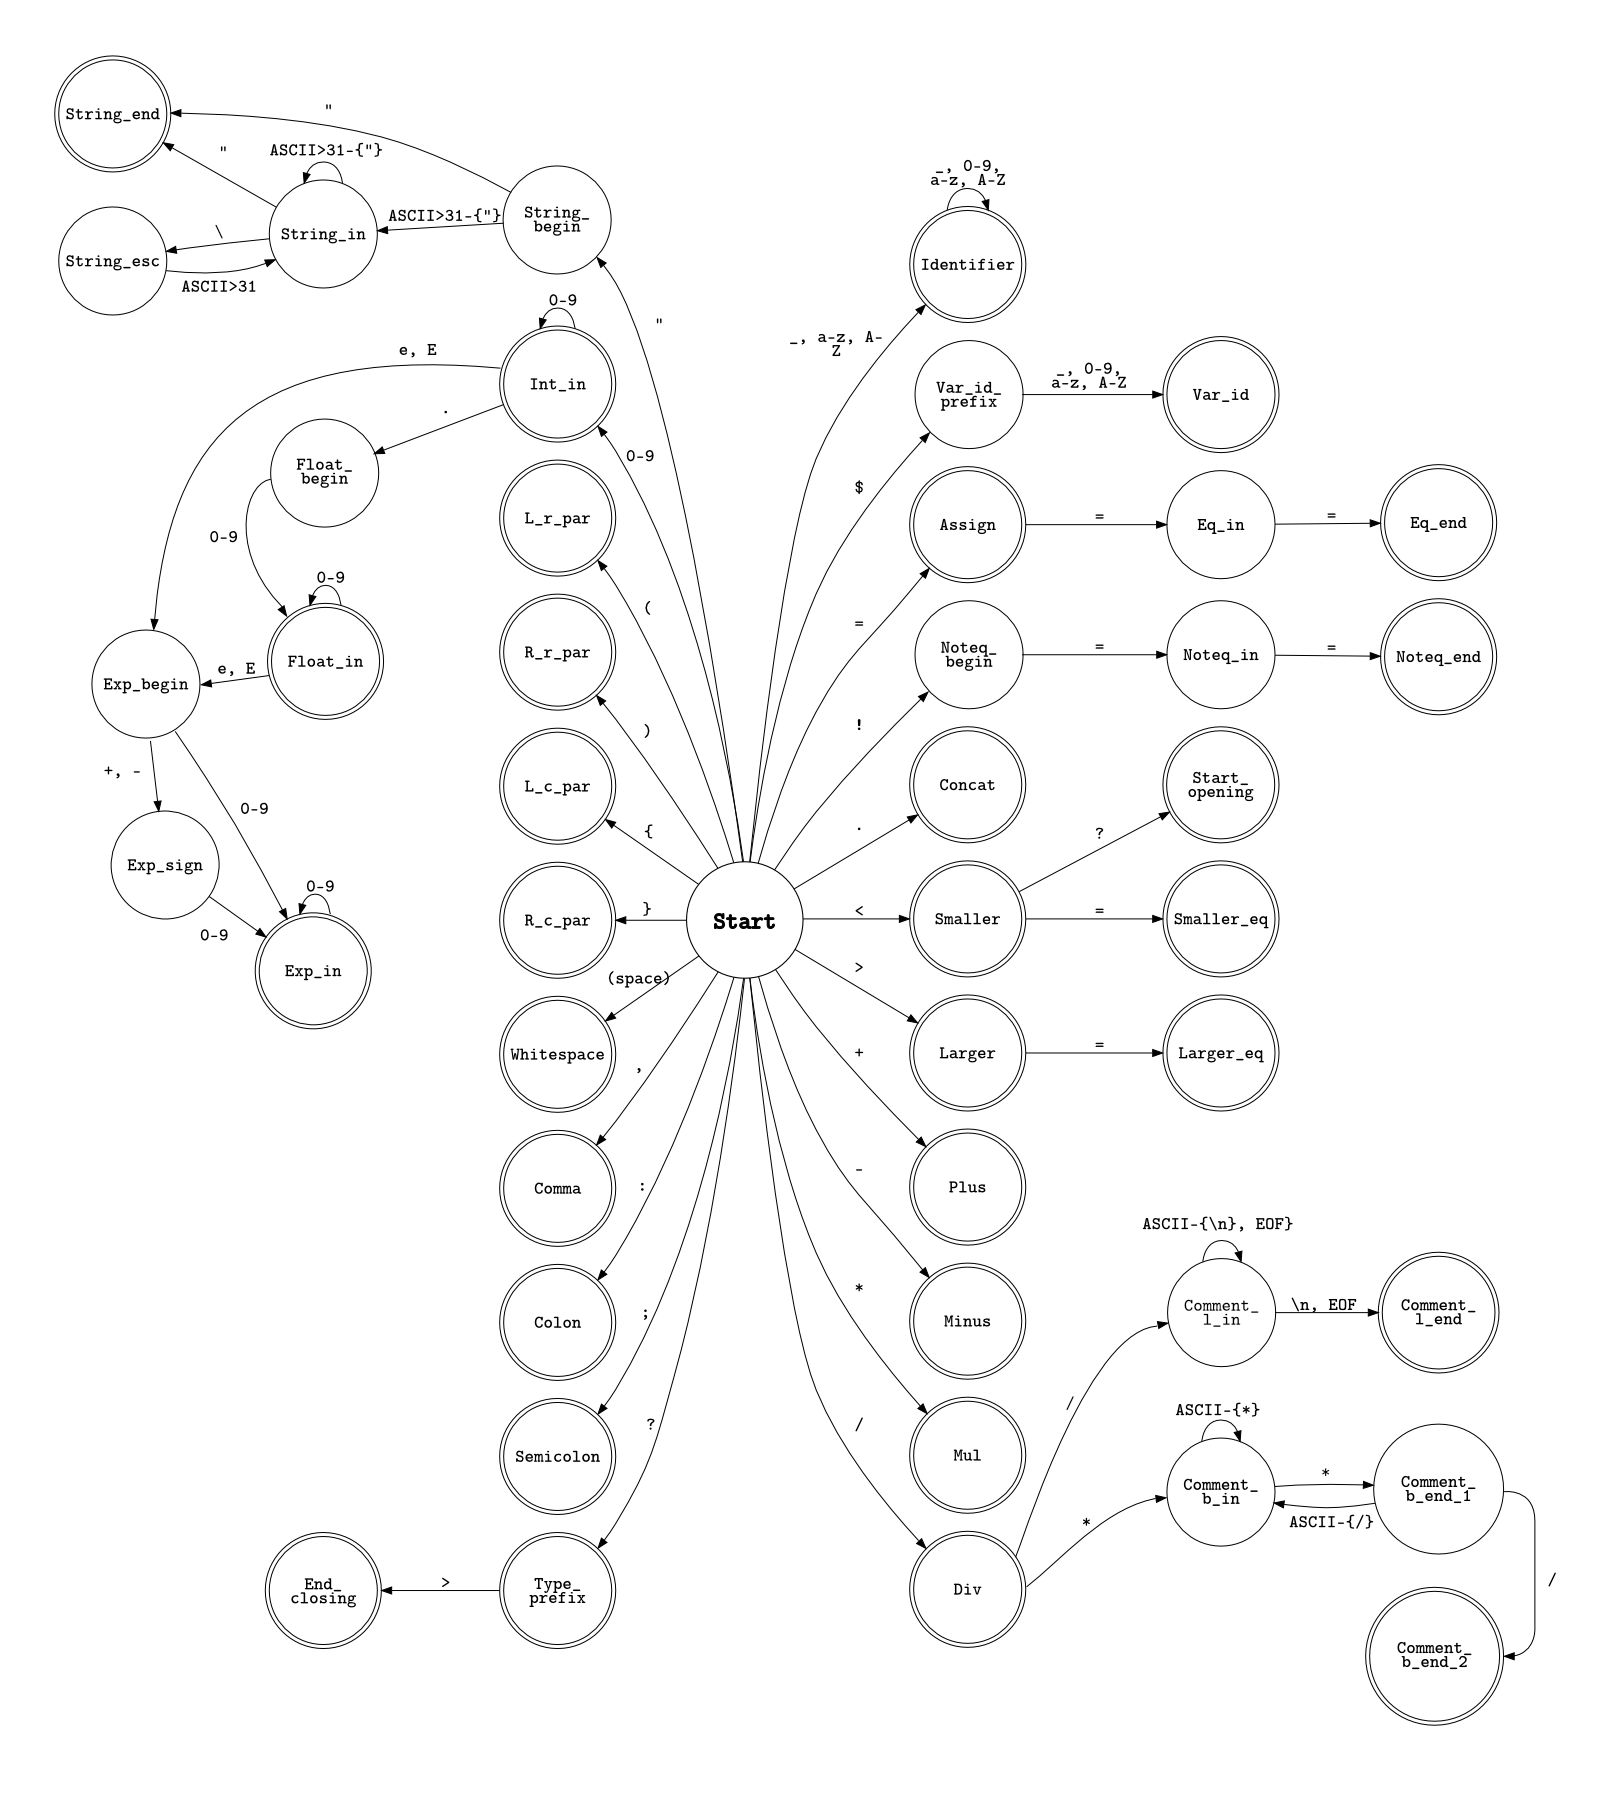
\includegraphics[width=1.2\textwidth]{include/fsm.png}}
	\caption{Diagram konečného automatu vytvořený nástrojem \texttt{Graphviz}}
\end{figure}

\pagebreak{}
    
\section{Syntaktická analýza}
    
\subsection{Implementace}
Implementace syntaktické analýzy je obsažena v souborech \verb|parser.c| a \verb|parser.h|.
\\ \\
Hlavní funkce syntaktického analyzátoru je \verb|parser()|. Parametrem dostává ukazatel na seznam tokenů,
se kterými pracuje, a pro účely sémantické analýzy ukazatel na strukturu tabulek symbolů a číslo průchodu.
Funkce \verb|parser()| nejprve kontroluje správnost prologu. Ten kontroluje funkce \verb|checkProlog|, která
prochází tokeny prologu a v případě chyby vrací chybový kód 1. \\\\
Pro začátek syntaktické analýzy je volána funkce \verb|rule_Prog|, jedna z funkcí reprezentující neterminály gramatiky.
Pro každý neterminál existuje funkce, která na základětypu následujícího tokenu pravidlo, které se pro zpracování použije.\\\\
Na základě pravidel LL-gramatiky a LL-tabulky funkce \verb|parser()| vybírá podle typu následujícího tokenu pravidlo,
které se pro zpracování použije.\\\\
Postupně se zpracovávají terminály, které zpracovává funkce \verb|parseTerminal()|, jejíž parametr typu tokenu určuje typ tokenu,
který by měl být další. Pokud není očekávaný typ, vrací chybu. Pokud se narazí na neterminál, je volaná funkce pro tento neterminál.
Zpracovávání probíhá dokud není načten token typu \verb|EOF|, tedy konec souboru.

\subsection{Precedenční analýza}
Precedenční analýza je řešena v \verb|exp_parser.c| a má rozhraní v \verb|exp_parser.h|. Obsahuje 2 funkce.
\newline Funkce \verb|parse_expression_with_tree()| slouží k syntaktické kontrole výrazů a sestavení parsovacího stromu, který se sestaven na základě precedence operátorů se kterým dále pracuje generátor kódu. Funkce \verb|exp_parser()| slouží čistě ke zpřehlednění kódu. Implementace je dále doplněna o funkci \verb|precedence()| která vrací prioritu operátoru.

\subsection{Syntaktický strom}
Syntaktický strom je implementován v \verb|parse_tree.c| se stejnojmeným rozhraním. Nejdůležitější je funkce \verb|makeOpNode()|, která vytvoří strom s operátorem v kořenovém uzlu a 2 potomky jako operandy. \verb|printPtree()| je pak dále využívána generátorem kódu viz sekce 6. Zbytek funkcí slouží pro vkládání nových uzlů a pro alokování a uvolňování zdrojů.

\pagebreak{}
\subsection{LL-gramatika}
Pro jazyk IFJ22 byla navržena následující gramatika.
\begin{Verbatim}
	1:  <prog> -> <stat> <prog>
	2:  <prog> -> function func-id ( <params> ) : type { <st-list> } <prog>
	3:  <prog> -> <eof>
		
	4:  <eof> -> ?> EOF
	5:  <eof> -> EOF
		
	6: <params-cont> -> , type $id <params-cont>
	7: <params-cont> -> eps
		
	8: <params> -> type $id <params-cont>
	9: <params> -> eps
		
	10: <args-cont> -> , <term> <args-cont>
	11: <args-cont> -> 
		
	12: <args> -> <term> <args-cont>
	13: <args> -> eps
		
	14: <stat> -> $id = <assign> ;
	15: <stat> -> while ( <expr> ) { <st-list> }
	16: <stat> -> if ( <expr> ) { <st-list> } else { <st-list> }
	17: <stat> -> return <expr> ;
	18: <stat> -> <expr> ;
	19: <stat> -> func-id ( <args> ) ;
		
	20: <st-list> -> <stat> <st-list>
	21: <st-list> -> eps
		
	22: <assign> -> <expr>
	23: <assign> -> func-id ( <args> )
		
	24: <term> -> $id
	25: <term> -> val
\end{Verbatim}
\subsection*{Poznámky}
\texttt{\$id} - identifikátor proměnné\\
\texttt{func-id} - identifikátor funkce\\
\texttt{val} - číselný nebo řetězcový literál \\
\texttt{type} - datový typ (\texttt{int}, \texttt{double}, \texttt{string}, \texttt{void} \\
\texttt{func-id} - identifikátor funkce \\
\texttt{eps} - $\varepsilon$ \\

\subsection{LL-tabulka}

\renewcommand{\familydefault}{\ttdefault}

\begin{table}[H]
	\makebox[\textwidth][c]{
		\begin{tabular}{|l|l|l|l|l|l|l|l|l|l|l|l|l|l|l|l|l|l|l|l|l|}
			\hline
			& \textbf{\begin{sideways}function   \ \end{sideways}}
			& \textbf{\begin{sideways}func-id\end{sideways}}   
			& \textbf{\begin{sideways}(\end{sideways}}
			& \textbf{\begin{sideways})\end{sideways}}
			& \textbf{\begin{sideways}:\end{sideways}}
			& \textbf{\begin{sideways}type\end{sideways}}
			& \textbf{\begin{sideways}\{\end{sideways}}
			& \textbf{\begin{sideways}\}\end{sideways}}
			& \textbf{\begin{sideways}?\textgreater{}\end{sideways}}
			& \textbf{\begin{sideways}EOF\end{sideways}}
			& \textbf{\begin{sideways},\end{sideways}}
			& \textbf{\begin{sideways}\$id\end{sideways}}
			& \textbf{\begin{sideways}=\end{sideways}}
			& \textbf{\begin{sideways}; \end{sideways}}
			& \textbf{\begin{sideways}while \end{sideways}}
			& \textbf{\begin{sideways}\textless{}expr\textgreater{}\end{sideways}}
			& \textbf{\begin{sideways}if\end{sideways}}
			& \textbf{\begin{sideways}else\end{sideways}}
			& \textbf{\begin{sideways}return\end{sideways}}
			& \textbf{\begin{sideways}val\end{sideways}} \\ \hline
			\textbf{\textless{}prog\textgreater{}}        & 2 & 1  &   &    &   &   &   &    & 3 & 3                                      &    & 1  &   &   & 1  & 1  & 1  &   & 1  &                                       \\ \hline
			\textbf{\textless{}eof\textgreater{}}         &   &    &   &    &   &   &   &    & 4 & 5                                      &    &    &   &   &    &    &    &   &    &                                       \\ \hline
			\textbf{\textless{}params-cont\textgreater{}} &   &    &   & 7  &   &   &   &    &   &                                        & 6  &    &   &   &    &    &    &   &    &                                       \\ \hline
			\textbf{\textless{}params\textgreater{} }     &   &    &   & 9  &   & 8 &   &    &   &                                        &    &    &   &   &    &    &    &   &    &                                       \\ \hline
			\textbf{\textless{}args-cont\textgreater{}}   &   &    &   & 11 &   &   &   &    &   &                                        & 10 &    &   &   &    &    &    &   &    &                                       \\ \hline
			\textbf{\textless{}args\textgreater{} }       &   &    &   & 13 &   &   &   &    &   &                                        &    & 12 &   &   &    &    &    &   &    & 12                                    \\ \hline
			\textbf{\textless{}stat\textgreater{}  }      &   & 19 &   &    &   &   &   &    &   &                                        &    & 14 &   &   & 15 & 18 & 16 &   & 17 &                                       \\ \hline
			\textbf{\textless{}st-list\textgreater{}   }  &   & 20 &   &    &   &   &   & 21 &   &                                        &    & 20 &   &   & 20 & 20 & 20 &   & 20 &                                       \\ \hline
			\textbf{\textless{}assign\textgreater{}   }   &   & 23 &   &    &   &   &   &    &   &                                        &    &    &   &   &    & 22 &    &   &    &                                       \\ \hline
			\textbf{\textless{}term\textgreater{}    }    &   &    &   &    &   &   &   &    &   &                                        &    & 24 &   &   &    &    &    &   &    & 25                                    \\ \hline
		\end{tabular}}
	\renewcommand{\familydefault}{\sfdefault}
\end{table}
\renewcommand{\familydefault}{\sfdefault}
\begin{center}
	\caption{Obrázek 2: LL-tabulka s pravidly přechodů}
\end{center}

\subsection{Precedenční tabulka}
\renewcommand{\familydefault}{\ttdefault}

\begin{table}[H]
	\makebox[\textwidth][c]{
		\begin{tabular}{|l|c|c|c|c|c|c|c|c|c|c|c|c|c|c|c|}
			\hline
			                         & \textbf{*}     & \textbf{/}     & \textbf{+}     & \textbf{-}     & \textbf{.}     & \textbf{\textless{}} & \textbf{\textgreater{}} & \textbf{\textless{}=} & \textbf{\textgreater{}=} & \textbf{===}   & \textbf{!==}   & \textbf{(}  & \textbf{)}     & \textbf{var} & \textbf{\$}    \\ \hline
			\textbf{*}               & \textgreater{} & \textgreater{} & \textgreater{} & \textgreater{} & \textgreater{} & \textgreater{}       & \textgreater{}          & \textgreater{}        & \textgreater{}           & \textgreater{} & \textgreater{} & \textless{} & \textgreater{} & \textless{} & \textgreater{} \\ \hline
			\textbf{/}               & \textgreater{} & \textgreater{} & \textgreater{} & \textgreater{} & \textgreater{} & \textgreater{}       & \textgreater{}          & \textgreater{}        & \textgreater{}           & \textgreater{} & \textgreater{} & \textless{} & \textgreater{} & \textless{} & \textgreater{} \\ \hline
			\textbf{+}               & \textless{}    & \textless{}    & \textgreater{} & \textgreater{} & \textgreater{} & \textgreater{}       & \textgreater{}          & \textgreater{}        & \textgreater{}           & \textgreater{} & \textgreater{} & \textless{} & \textgreater{} & \textless{} & \textgreater{} \\ \hline
			\textbf{-}               & \textless{}    & \textless{}    & \textgreater{} & \textgreater{} & \textgreater{} & \textgreater{}       & \textgreater{}          & \textgreater{}        & \textgreater{}           & \textgreater{} & \textgreater{} & \textless{} & \textgreater{} & \textless{} & \textgreater{} \\ \hline
			\textbf{.}               & \textless{}    & \textless{}    & \textgreater{} & \textgreater{} & \textgreater{} & \textgreater{}       & \textgreater{}          & \textgreater{}        & \textgreater{}           & \textgreater{} & \textgreater{} & \textless{} & \textgreater{} & \textless{} & \textgreater{} \\ \hline
			\textbf{\textless{}}     & \textless{}    & \textless{}    & \textless{}    & \textless{}    & \textless{}    & \textgreater{}       & \textgreater{}          & \textgreater{}        & \textgreater{}           & \textgreater{} & \textgreater{} & \textless{} & \textgreater{} & \textless{} & \textgreater{} \\ \hline
			\textbf{\textgreater{}}  & \textless{}    & \textless{}    & \textless{}    & \textless{}    & \textless{}    & \textgreater{}       & \textgreater{}          & \textgreater{}        & \textgreater{}           & \textgreater{} & \textgreater{} & \textless{} & \textgreater{} & \textless{} & \textgreater{} \\ \hline
			\textbf{\textless{}=}    & \textless{}    & \textless{}    & \textless{}    & \textless{}    & \textless{}    & \textgreater{}       & \textgreater{}          & \textgreater{}        & \textgreater{}           & \textgreater{} & \textgreater{} & \textless{} & \textgreater{} & \textless{} & \textgreater{} \\ \hline
			\textbf{\textgreater{}=} & \textless{}    & \textless{}    & \textless{}    & \textless{}    & \textless{}    & \textgreater{}       & \textgreater{}          & \textgreater{}        & \textgreater{}           & \textgreater{} & \textgreater{} & \textless{} & \textgreater{} & \textless{} & \textgreater{} \\ \hline
			\textbf{===}             & \textless{}    & \textless{}    & \textless{}    & \textless{}    & \textless{}    & \textless{}          & \textless{}             & \textless{}           & \textless{}              & \textgreater{} & \textgreater{} & \textless{} & \textgreater{} & \textless{} & \textgreater{} \\ \hline
			\textbf{!==}             & \textless{}    & \textless{}    & \textless{}    & \textless{}    & \textless{}    & \textless{}          & \textless{}             & \textless{}           & \textless{}              & \textgreater{} & \textgreater{} & \textless{} & \textgreater{} & \textless{} & \textgreater{} \\ \hline
			\textbf{(}               & \textless{}    & \textless{}    & \textless{}    & \textless{}    & \textless{}    & \textless{}          & \textless{}             & \textless{}           & \textless{}              & \textless{}    & \textless{}    & \textless{} & =              & \textless{} &                \\ \hline
			\textbf{)}               & \textgreater{} & \textgreater{} & \textgreater{} & \textgreater{} & \textgreater{} & \textgreater{}       & \textgreater{}          & \textgreater{}        & \textgreater{}           & \textgreater{} & \textgreater{} &             & \textgreater{} &             & \textgreater{} \\ \hline
			\textbf{var}             & \textgreater{} & \textgreater{} & \textgreater{} & \textgreater{} & \textgreater{} & \textgreater{}       & \textgreater{}          & \textgreater{}        & \textgreater{}           & \textgreater{} & \textgreater{} &             & \textgreater{} &             & \textgreater{} \\ \hline
			\textbf{\$}              & \textless{}    & \textless{}    & \textless{}    & \textless{}    & \textless{}    & \textless{}          & \textless{}             & \textless{}           & \textless{}              & \textless{}    & \textless{}    & \textless{} &                & \textless{} &                \\ \hline
		\end{tabular}}
	    
\end{table}
\renewcommand{\familydefault}{\sfdefault}
\begin{center}
	\caption{Obrázek 3: Precedenční tabulka pro práci s výrazy}
\end{center}

\pagebreak{}

\section{Sémantická analýza}
Sémantická analýza probíhá v souborech \verb|parser.c| a \verb|parser_tree.c| ve formě různě rozmístněných kontrol. 
\subsection{Nedefinování/redefinováni funkce}
Název funkce, kterou kontrolujeme, si ukládáme v globální proměnné \verb|functionName|. Ten se vyhledává v tabulce symbolů, nebo se porovnává s názvy vestavěných funkcí. Pokud jde o neexistující funkci, nebo o redefinici už existující funkce, ukončíme program s návratovou hodnotou 3.
\subsection{Argumenty a návratová hodnota funkce}
Počet parametrů funkce a typ její návratové hodnoty si při definici funkce ukládáme do tabulky symbolů. Při použití zadefinované funkce později v programu počítáme počet argumentů, s kterými jsme funkci zavolali.  Vyjímkou je však vestavěná funkce \verb|write|, která má libovolný počet parametrů. Kontrola typu návratové hodnoty probíhá vygenerováním příkazů v cílovém jazyku, který porovnává typ hodnoty, kterou má funkce vracet, a typ hodnoty, kterou skutečně vrací. Tato kontrola proběhne až při spuštění kódu vygenerovaného překladačem. Kontrolujeme i zda ve funkcích nechybí příkaz \verb|return| za pomoci globální proměnné \verb|hasReturn|, pokud v sobě tato proměnná má uloženou hodnotu false a zároveň funkce, kterou definujeme, nemá návratový typ \verb|void|, potom, stejně jako s ostatními kontrolami, ukončíme program s návratovou hodnotou 4.
\subsection{Použití nedefinované proměnné}
Kontrola použití nedefinovanné proměnné probíhá v souboru \verb|parser_tree.c|. Když ve výrazu používáme proměnnou, vyhledáme jí v tabulce symbolů. Pokud jí nenajdeme, program se ukončí s návratovou hodnotou 5.
\subsection{Chybějící/přebývající výraz v návratu z funkce}
Při použití příkazu \verb|parser_tree.c|, skontrolujeme, jaký návratový typ má funkce, v které příkaz používáme, pokud má návratový typ \verb|void| a při příkazu \verb|return| se nachází výraz, ukončíme program s chybou 6. Stejně ukončíme program, pokud funkce nemá navratový typ \verb|void| a při příkazu \verb|return| výraz chybí.

\pagebreak{}

\section{Tabulka symbolů}
Tabulka symbolů je implementována v souborech \verb|symtable.c| a \verb|symtable.h| jako  tabulka symbolů s rozptýlenými položkami.
\subsection{Rozptylovací funkce}
Je použita varianta pro sdbm s magickou konstantou \boldsymbol{65 599}. Jak funkce tak i konstanta jsou převzaty z předmětu IJC vyučovaného v letním semestru 2021/22.
\footnote{ Stránka předmětu IJC: \url{http://www.fit.vutbr.cz/study/courses/IJC/public/DU2.html.cs}}
\footnote{ Popis sdbm: \url{http://www.cse.yorku.ca/~oz/hash.html}}

\subsection{Typy a struktury}
Tabulka symbolů využívá typu \verb|symtable_t| což je struktura obsahující struktury symbolů typu \verb|symbol_t|. Symboly pak obsahují potřebné informace pro definice, generov vyhodnocování výrazů a sémantickou analýzu. Další typ \verb|symtables_t| pak slouží pro uchování tabulek symbolů pro funkce, proměnné a pro pohodlnou práci s rámci. 
\subsection{Funkce}
Tabulka musí z tokenů používané v syntaktické analýze udělat symboly. Na to slouží funkce \verb|token_to_symbol()|.
Tabulka symbolů je dynamicky alokována a její implementace obsahuje funkce na kontrolu velikosti, její následné zvětšení a další pomocné funkce pro prácí s tabulkou(insert, print,...). 

\pagebreak{}

\section{Generování kódu}
Generování kódu probíhalo v modulech syntaktického parseru a parseru pro výrazy. Kód se nachází v jednotlivých funkcích a generuje se postupně s jejích voláním, tj. postupně s průchodem syntaktického parseru.
\subsection{Práce s tabulkou symbolů}
Pro správné generování bylo potřeba využít tabulky symbolů, do které se při prvním průchodu uloží proměnné a na začátku hlavního těla a na začátku těla každé funkce se vygenerují definice proměnných naležících pro danné tělo. Nekompletní kód vygenerovaný prvním průchodem se přeskočí pomocí instrukce \verb|JUMP| a za správný se považuje až kód z druhého průchodu.
\subsection{Generování kódu pro výrazy}
Generování kódu probíhá při Inorder průchodu binárním stromem vygenerovaných precedenční analýzou. Zároveň se tiskne kód, který sám o sobě umí zkontrolovat, jestli operace, které provádíme jsou validní a mají správné operandy. 
\subsection{Konverze typů pro výrazy v podmínce a cyklu}
Cykly a podmínky jsou řešené pomocí porovnávání s hodnotou \verb|bool@false|, proto bylo potřeba nejprve převést výsledek z generování výrazu na tento typ. Převádění hodnoty se provádí až v IFJcode22 kódu, který se generuje, když parser narazí na podmínku nebo cyklus.
    
\subsection{Vestavěné funkce}
Vestavěné funkce jazyka \verb|IFJ22| byly přímo napsány v cílovém jazyku \verb|IFJcode22| a tisknou se na konci kódu vygenerovaného překladačem.

\pagebreak{}

\section{Hlavní program}
Hlavní program obsahuje soubor \verb|main.c|. Hlavní program nejprve plní strukturu tokenů voláním funkce lexeru \verb|FillTokenList()|.
Následovně se vytvoří veškeré potřebné tabulky symbolů, které se používají v syntaktické a sémantické analýze. Spustí se první průchod funkce \verb|parser()|,
který zajistí naplnění tabulky symbolů indetifikátory funkcí a proměnných, poté se spouští druhý průchod, který už kontroluje správnou sémantiku.
Na konec je tištěn kód pro vestavěné funkce. Po vykonání překladu je uvolněna alokovaná pamět pro tabulky symbolů a vázaný seznam tokenů.
Pokud je hlavnímu programu v nějaké fázi vrácen chybový kód, je program ukončen s náležitým chybovým kódem a hláškou typu chyby.

\section{Členění implementačního řešení}
Jednotlivé části programu jsou rozděleny do zdrojových souborů následovně.
\begin{itemize}
	\item\texttt{error.c/h} - Chybové výpisy a kódy
	\item\texttt{exp\_parser.c/h} - Zpracování výrazů
	\item\texttt{lexer.c/h} - Lexikální analyzátor
	\item\texttt{main.c} - Hlavní program
	\item\texttt{parser.c/h} - Syntaktický a sémantický analyzátor, generování kódu
	\item\texttt{parse\_tree.c/h} - Abstraktní syntaktický strom pro práci s výrazy
	\item\texttt{stack.c/h} - Zásobník
	\item\texttt{symtable.c/h} - Tabulka symbolů implementovaná jako tabulka s rozptýlenými prvky
\end{itemize}

\end{document}
